\chapter*{Proposition 48}



\begin{figure*}[ht]
    \begin{center}
    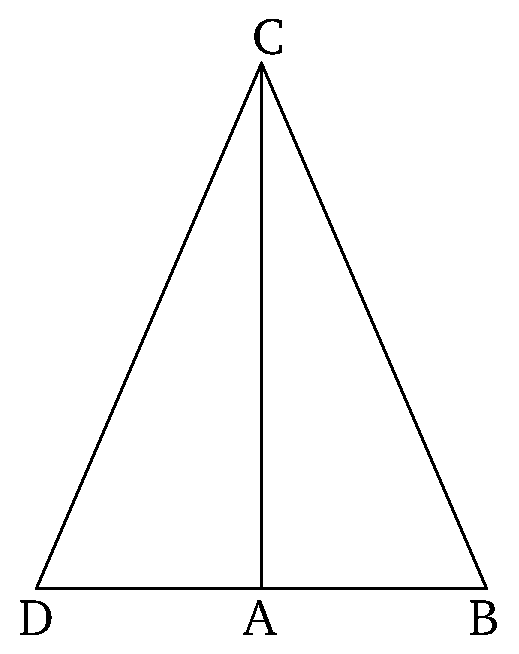
\includegraphics[width=0.5\linewidth]{figures/fig48e.eps}
    \label{fig:prop_48}
    \end{center}
\end{figure*}


If the square on one of the sides of a triangle is equal to the (sum of the)
squares on the two remaining sides of the triangle then the angle contained
by the two remaining sides of the triangle is a right-angle.

For let the square on one of the sides, $BC$, of triangle $ABC$ be equal
to the (sum of the) squares on the sides $BA$ and $AC$. I say that angle
$BAC$ is a right-angle.

For let $AD$ have been drawn from point $A$ at right-angles to the
straight-line $AC$ [Prop.~1.11], and let $AD$ have been made equal to
$BA$ [Prop.~1.3], and let $DC$ have been joined. Since $DA$ is equal to $AB$,
the square on $DA$ is thus also equal to the square on $AB$.$^\dag$ Let the square on
$AC$ have been added to both. Thus, the (sum of the) squares on $DA$ and $AC$ is equal
to the (sum of the) squares on $BA$ and $AC$. But, the (square) on $DC$ 
is equal to the (sum of the squares) on $DA$ and $AC$. For angle $DAC$ is a right-angle [Prop.~1.47].
But, the  (square) on $BC$ is equal to (sum of the squares) on $BA$ and $AC$.
For (that) was assumed. Thus, the square on $DC$ is equal to the square on $BC$.
So  side $DC$ is also equal to (side) $BC$. And since $DA$ is equal to $AB$, and $AC$ (is) common, the two (straight-lines) $DA$, $AC$ are equal to the two (straight-lines)
$BA$, $AC$. And the base $DC$ is equal to the base $BC$. Thus, angle $DAC$ [is] equal to angle $BAC$ [Prop.~1.8].  But $DAC$ is a right-angle. Thus, $BAC$ is
also a right-angle.

Thus, if the square on one of the sides of a triangle is equal to the (sum of the)
squares on the remaining two sides of the triangle then the angle contained
by the remaining two sides of the triangle is a right-angle. (Which is) the very thing
it was required to show.


\section*{Commentary}

\begin{proposition}\label{proposition_48}\lean{Elements.Book1.proposition_48}\leanok
    If
\end{proposition}
\begin{proof}
    \uses{proposition_3,proposition_8,proposition_11,proposition_47}\leanok
\end{proof}
